% This is samplepaper.tex, a sample chapter demonstrating the
% LLNCS macro package for Springer Computer Science proceedings;
% Version 2.20 of 2017/10/04
%
\documentclass[runningheads]{llncs}
%
\usepackage{graphicx}
% Used for displaying a sample figure. If possible, figure files should
% be included in EPS format.
%
% If you use the hyperref package, please uncomment the following line
% to display URLs in blue roman font according to Springer's eBook style:
% \renewcommand\UrlFont{\color{blue}\rmfamily}

\begin{document}
%
\title{Subtle Gestures with the J!NS MEME}
%
%\titlerunning{Abbreviated paper title}
% If the paper title is too long for the running head, you can set
% an abbreviated paper title here
%
\author{Thomas Bartel \and
Florian Bossert \and
Sajjad Ahmad}
%
% TODO should we use 'et al.' here? ~FB
\authorrunning{T. Bartel \and F. Bossert \and S. Ahmad}
% First names are abbreviated in the running head.
% If there are more than two authors, 'et al.' is used.
%
\institute{Karlsruhe Institute of Technology, Karlsruhe, Germany}
%
\maketitle              % typeset the header of the contribution
%
\begin{abstract}
The abstract should briefly summarize the contents of the paper in
15--250 words.

\keywords{First keyword  \and Second keyword \and Another keyword.}
\end{abstract}
%
%
%
\section{Introduction}
\subsection{A Subsection Sample}
Please note that the first paragraph of a section or subsection is
not indented. The first paragraph that follows a table, figure,
equation etc. does not need an indent, either.

Subsequent paragraphs, however, are indented.

% As a reference, maybe useful later
Current smartglasses:
Smartglasses with cameras: Spectacles by Snap Inc. https://www.spectacles.com/
Smartglasses with EOG sensors: J!ns Meme by J!ns (website currently only in Japanese):
https://jins-meme.com/

% Assigned to FB
\section{Related Work}
Our work touches on multiple areas of research, including wearable sensing, gesture
recognition, and subtle interaction. In the following section we roughly outline
previous works in these areas.

\subsection{The Human Body as an Input Interface}
There are various works discussing the use of the human body as an input interface, with
most of them having an exploratory nature:
Harrison et al. resolved the location of finger tapping on the user's arm and hand
using acoustic sensing \cite{10.1145/1753326.1753394}.
Serrano et al. explored Hand-to-Face input by tracking infrared markers applied to
fingers with an optical system \cite{10.1145/2556288.2556984}.
Lisserman et al. proposed the human ear as an input surface, which can be used by
touching it in certain ways. This was achieved by placing electrodes around the ear
\cite{10.1145/2468356.2468592}.
Even eyelid gestures have been looked into by Jota et al., who developed a framework
and prototypes for them \cite{10.5555/2788890.2788938}.
Using a battery-free low-power wrist band, Truong et al. managed to classify hand
gestures by detecting skin deformations \cite{10.1145/3274783.3274854}.

Especially when using extremities as input methods, inertial measurement units (IMUs),
which consist of accelerometers and gyroscopes, have been widely employed: Wen et al.
used them to recognize unremarkable fine-motor finger movements
\cite{10.1145/2858036.2858466}. Laput et al. utilized the IMUs in commercially available
smartwatches with a custom performance-boosting kernel to classify a wide variety of hand
gestures \cite{10.1145/2984511.2984582}.

As for applications of wearable sensing, there are many from convenient user input
to medical monitoring:
Ike et al. demonstrated using hand gestures to control a TV's content navigation interface
with a IMU-equipped wrist band \cite{10.1145/2641248.2641359}.
Ohnishi et al. used sensors in shoes to track exercises and general posture
\cite{10.1145/3174910.3174938}.
Schiboni et al. monitored drinking with wrist-worn inertial sensors, demonstrating
the feasibility of long-term sparse natural gesture recognition
\cite{10.1145/3267242.3267253}.
On the more medical side, Milosevic et al. performed jump performance analysis with
low-cost wearable devices instead of pressure-sensitive force plates, with the intent
of making training progress monitoring more easily available \cite{10.1145/2753509.2753512}.
Again for automatic monitoring, Bedri et al. used wearable sensors to track
eating episodes instead of making patients rely on often biased self-written food intake
journals \cite{10.1145/3130902}.

\subsection{EOG Sensing and Subtle Interaction}
While the aforementioned work utilized mainly IMUs, touch sensors or optical systems,
Electrooculography (EOG) has become a useful tool for eye-tracking in recent years, too. 
In 2006, Manabe et al. attached EOG sensors to over-ear \cite{10.1145/1125451.1125655}
and in 2013, to in-ear head phones \cite{10.1145/2493988.2494329} to detect eye gestures.
Bulling et al. first demonstrated efficient real-time eye-movement recognition
with EOG goggles in 2009, which they custom-made \cite{10.1145/1520340.1520468}.
Once commercial EOG glasses became available in 2014, Ichimaru et al. used them for
activity recognition \cite{10.1145/2638728.2638795}. They used the J!ns Meme
smartglasses to distinguish between typing, reading, eating and talking.
As for more recent work, Li et al. used the J!ns Meme to infer the physical and social
context of the wearer by recognizing various greeting gestures involving kissing
\cite{10.1145/3384657.3384801}.

In contrast to the work discussed, which often employed noticable or obviously unusual
hardware, we explicitly focus on subtle interaction. Pohl et al. define
four types of subtle interaction: (1) signifying feedback that is non-intrusive to the
user, (2) hiding interaction from others and potentially deceiving them, (3) employing
less effort for input and generally doing less, and (4) nudging users
\cite{10.1145/3290605.3300648}. Our work aims at type (2) social subtlety, like e.g.
Ashbrook et al. did with their tooth-click gesture recognition interface
\cite{10.1145/2935334.2935389}. With a similar goal, Li et al. developed TongueBoard,
a retainer form-factor device for recognizing silent speech \cite{10.1145/3311823.3311831}.

Itchy Nose by Lee et al. is the most closely related work to ours,
as it inspired our efforts \cite{10.1145/3123021.3123060}. They used the J!ns Meme
smartglasses to detect multiple gestures that consisted of rubbing or pushing their
noses, which can also be detected by the glasses' EOG sensors.

% Assigned to FB
\section{Analysis}
% TODO introduction for analysis section
What does our research contribute? (Additional subtle gestures, ...)

% TODO, maybe do this in the Introduction section? ~FB
Explaining the J!ns Meme.

% TODO
What was our goal?

\subsection{Workflow}
We began with planning the rough outline that our research would follow.
The plan was as follows:
\begin{itemize}
    \item Gather gesture ideas
    \item Check ideas for detectable responses
    \item Create tools to automate the recording of gestures
    \item Collect labelled data with the tools
    \item Model, train and validate a neural network until its performance is sufficient
    \item Test the network on our withheld test dataset
\end{itemize}

[Insert figure here]

\subsection{Gestures}
% TODO, maybe use self-made illustrations here
In the first phase, we came up with gestures we considered subtle. Early candidates were:
\begin{itemize}
    \item Pushing your glasses up your nose [see GIF]
    \item A thinking pose, where you touch your chin with your thumb and your cheek with your
        index finger [see GIF]
    \item Slow nodding [see GIF]
    \item Tapping the frame of the glasses [see GIF]
\end{itemize}

Since some of the gestures generated barely any responses on the EOG or the IMU readouts
[see figures with an example of a strong and a weak response],
we continued coming up with gestures until we had a total of seven gestures.
The gestures we came up with and their apparent responses can be seen in table \ref{responses}.

\begin{table}
\caption{The quality of the EOG and IMU sensor responses for our gestures.}\label{responses}
\begin{tabular}{|l|l|}
    \hline
    Gesture description & Response quality\\
    \hline
    Pushing glasses up the nose & strong\\
    Readjusting glasses & strong\\
    Thinking pose & weak\\
    Slow nodding & strong\\
    Tilting head sideways & strong\\
    Stroking mustache & weak\\
    Biting lip & weak\\
    Tapping on the nose & strong\\
    Rubbing the nose & strong\\
    Pushing cheek up with a finger & strong\\
    Tapping the glasses & strong\\\hline
\end{tabular}
\end{table}

\subsection{Tools for Recording and Labelling}
% is this something for the implementation section? ~FB
How does the J!ns Meme work and how do we use it?

What data do we collect, how and why?
Itchy Nose tool for automating personalization \cite{10.1145/3174910.3174953}.

\subsection{Neural Network Architecture and Training}
% again - how much of this belongs to implementation? ~FB

% Assigned to TB
\section{Implementation}

The following sections give a detailed description of our implementation process. In total we implemented four programs during our research concerning the J1ns meme glasses. In the first step we implemented a data collection tool that supported our test subjects during the collection and labeling process. As already described in our analysis section, we then decided to implement a neural network based on an LSTM architecture. After that we created a third program that uses several other machine learning techniques to predict the correct gestures by using the data from the J1ns meme. This was a necessary step to show that our new LSTM-based architecture is able to perform just as well or even outperform other already established machine learning techniques in this gesture prediction task. The last step of our implementation process was a program that uses real time data from the J1ns meme glasses to predict the gestures that a user performs.

\subsection{Data collection tool}

The prediction of gesture classes by using the J!ns meme data is a supervised classification task. This means that a large amount of labeled data is needed to train our LSTM-based neural network and the other machine learning techniques. One of our goals of this project was the creation of a neural network that achieves good results in the gesture prediction task regardless of which person is currently using the J1ns meme glasses. To achieve this goal, it was necessary for us to select a diverse group of people that each collect a part of our training data. In total we selected ? (noch einfügen) people for the collection task.
\par
In order to create useful data for the machine learning techniques, you first have to collect the gesture data and afterwards assign them the correct label. We unified this process by creating a data collection tool that automatically assigns the correct label to the data after each gesture that the test subject performs.
\begin{center}
\begin{figure}
\centerline{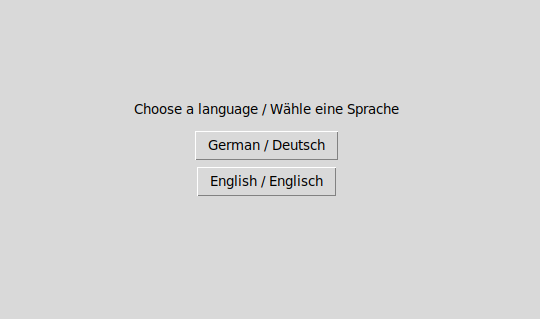
\includegraphics[scale=0.5]{Language_Selection.png}}
\caption{The language selection page of our data collection tool}
\label{fig:gesturestart}
\end{figure}
\end{center}
Figure \ref{fig:gesturestart} shows how the data collection tool lets the user choose a preferred language which is either german or english before the data collection starts. This language selection process is followed by a description of the experiment, which informs the user about what kind of data is collected and how the user is supposed to collect this data. These initial steps supply the user with all the important information that is needed to ensure a clean data collection process.
\par
After the initial steps the data collection process can start. We use a JSON file to configure which gestures the tool collects data for. Figure \ref{fig:gesturejson} shows an entry for the gesture PUSH\_GLASSES\_UP in the JSON file. For every gesture we define a name and description that is available in either english or german. The "sampleCount" specifies the amount of data samples our tool will collect for the defined gesture. We decided that 10 samples for each gesture is a good compromise between the time that is needed to finish the collection process and the amount of data that we receive for our task. The "label" is just the label that our tool assigns to the data samples of this gesture. This label is later used for our supervised classification task. The "file" entry is the name of an .mp4 file that shows an example of how this gesture is supposed to be performed. This type of configuration allows us to freely define any kind of gesture that the test subjects need to collect.
\begin{center}
\begin{figure}
\centerline{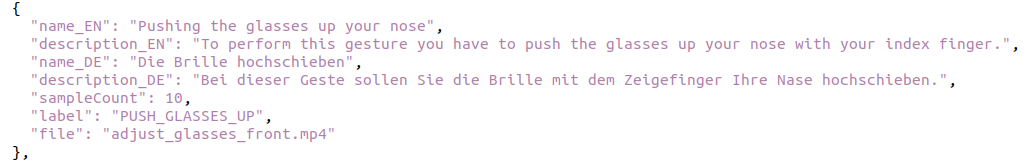
\includegraphics[width=\textwidth]{GestureJSON.png}}
\caption{A gesture defined in the JSON file of the data collection tool}
\label{fig:gesturejson}
\end{figure}
\end{center}

Figure \ref{fig:gesturedatacollection} shows how our tool asks a the user to collect data for a gesture. It shows a description of the gesture, how many samples of this type of gesture still need to be collected and a video that shows an exemplary execution of this type of gesture. As soon as the user is ready to perform this gesture, he can press the start button. In the next step the user needs to perform the described gesture. After he is finished the user needs to press the stop button. In the background our data collection tool saves the time when the start and when the stop button were pressed. This time interval is combined with the label that needs to be assigned to the data that was collect during this time. The triples of [label, start time, end time] allow us to automatically label the data that is collected from the J1ns meme during the collection process. The procedure gets repeated until every gesture that is defined in the JSON file has reached its defined sample count.
\begin{center}
\begin{figure}
\centerline{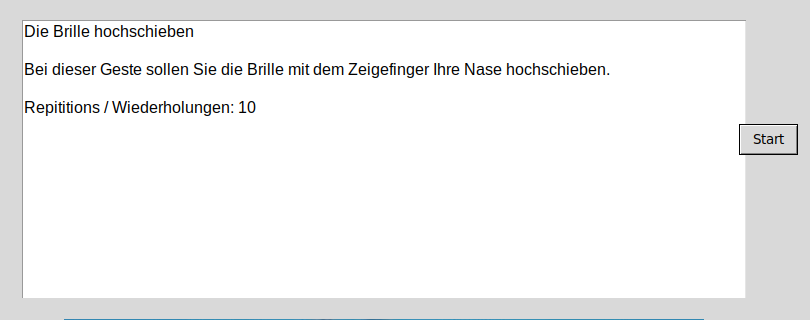
\includegraphics[scale=0.3]{Gesture_Description.png}}
\caption{The tool asks the test subject to collect data for a gesture}
\label{fig:gesturedatacollection}
\end{figure}
\end{center}

After a test subject finished the collection process, we extract the file with the data that was collected from the J!ns meme glasses. We created a script that uses the triples of [label, start time, end time] of our data collection tool to separate the collected data into files that only contain the data of a single gesture. After this step we are left with a fully labeled gesture dataset that can be used to train the different machine learning architectures.

\subsection{The LSTM-based neural network}

As already described in the analysis section of this paper we decided to use an LSTM-based architecture for our neural network because every gesture that is performed while wearing the J!ns meme glasses creates a stream of data. LSTM's use recurrent connections in their hidden states which allows them to remember information from previous timesteps which is ideal for our use case.
\par
For our implementation we made use of the pytorch library. The library consists of many already implemented features that are needed for the deep learning process. We especially made use of the pytorch LSTM implementation. To train our neural network we shuffled our automatically labeled gesture dataset and split it into three parts. We used 60\% of the data as our training dataset. Another 20\% was then used as our validation dataset that we used to tune our hyperparameters. The last 20\% was then used as a test dataset to see how good our network performs on unseen data.
\begin{center}
\begin{figure}
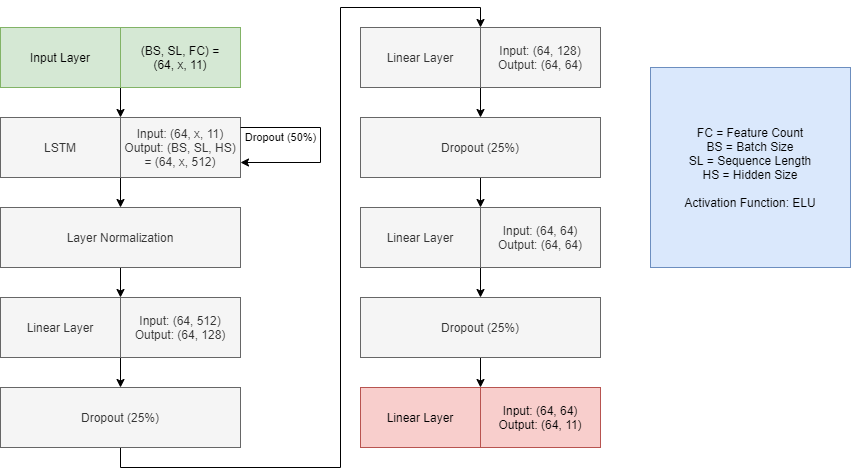
\includegraphics[width=\textwidth]{LSTM_Architecture.png}
\caption{The architecture of our LSTM-based neural network}
\label{fig:lstmarchitecture}
\end{figure}
\end{center}
Figure \ref{fig:lstmarchitecture} shows the complete architecture of our LSTM-based neural network.
\paragraph{Input layer}
Our input layers consists of the raw data stream of the J!ns meme glasses. During the training of the network the input has a shape of (64, x, 11). The first dimension is the batch size that we used during our training. We tested several different numbers and concluded that 64 was a good compromise between training time and performance. The second dimension is the sequence length of our input. Every gesture that is performed by a person is always unique which also means that the time, that is needed to perform a gesture is always different. That also means that the sequence length of a gesture is always a variable number. This is no problem in our use case because we decided to use an LSTM as the base of our neural network and they are especially made for sequences with variable length. The third dimension of the input is the feature count. In every timestep the J1ns meme produces a data vector that contains 11 features.
\paragraph{LSTM layer}
The input is then fed into an LSTM layer. This LSTM consists of 512 hidden states. We also tried several different hidden sizes for the LSTM and 512 was a good compromise between performance and training time. Small hidden sizes like 64 proved to be too small to completely learn our training data set while large hidden sizes like 1024 took too long to train. In our LSTM layer we used the built in dropout function of the pytorch library. We chose to use the standard dropout rate of 0.5 to prevent overfitting
\paragraph{Layer normalization}
The output of the LSTM layer is then put into a Layer normalization layer. This layer normalizes the LSTM output across the feature dimensions. This allows us to use higher learning rates, makes the network less dependent on weight initialization and introduces some noise to prevent overfitting.
\paragraph{Linear layers}
In the last step of our network we need to classify the output of our LSTM. For this task we use several stacked linear layers. Each linear layer gets progressively smaller until we reach the last layer that maps from a size of 64 to a size of 11 which is the amount of gestures that we trained our network for. Each layer except for the last one uses the Exponential Linear Unit acitvation function. The last layer uses the Softmax activation function which outputs pseudo probabilities for each of our gestures. During the test time the gesture that has the maximum probability gets assigned to the input. Between each linear layer we also used a dropout of 25\% to prevent our network from overfitting.

\subsection{Other machine learning techniques}

To be able to compare the performance of our LSTM-based neural network we implemented several other state of the art machine learning techniques and trained them with our dataset. To implement those machine learning techniques we made use of the scikit-learn python library. In total we implemented a Random Forest Classifier, a Decision Tree, a Naive Bayes Classifier, a Support Vector Machine and a K-Nearest Neighbor Classifier. The scikit-learn library already gave us access to standard implementations of those classifiers. These implementations all use a certain "fit()" function that automatically trains the classifier on a given dataset. One challenge that arose during the implementation of these classifiers was the preparation of the training dataset. While our LSTM-based neural network can easily deal with sequences of variable length, the other classifiers aren't naturally able to process them. If we look at our data then we can see that every gesture consists of several timesteps that each contain 11 feature values. We transformed each data sequence of a gesture into a large vector that has 11 x sequence length entries. We then padded every vector in the dataset with zeros in order for them to have the same length as the longest vector. These modifications allowed us to train the other classifiers with a dataset that consists of data sequences.

\subsection{Live gesture classification tool}

The final goal of our implementation was a tool that allows the live classification of gestures that are performed by a person wearing the J1ns meme glasses. Creating such a tool opens up the possibilities for applications that use these gestures to execute different types of commands. In order to gain access to the real time data that the J1ns meme glasses produce during their usage we use a built in function of the J1ns MEME Data Logger. This function writes the data to a specified IP-Adress and Port which allows us to write a tool that accesses the data on this port in real time.

\begin{center}
\begin{figure}
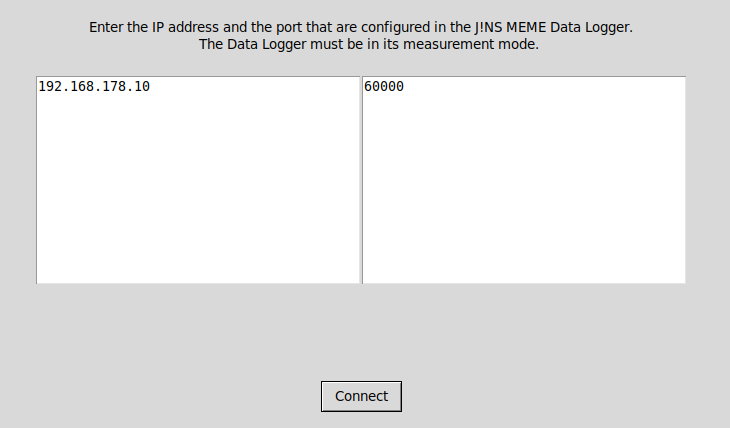
\includegraphics[width=\textwidth]{Live_Classification_IP.png}
\caption{The IP-address and port specification page}
\label{fig:ipandport}
\end{figure}
\end{center}

Figure \ref{fig:ipandport} shows the first page of our Live gesture classification tool. Here the user needs to specify the IP-address and the port that was specified in the J1ns MEME Data Logger. After the user presses the connect button the tool opens a new page where the live classification can start. We use the same procedure that we already used during our data collection process. To start the classification process the user has to press a start button. The tool then automatically records the time of this button press. Then the user performs the gesture. Afterwards he presses the stop button. The time for this button press is also automatically recorded by the tool. Now the tool tries to classify the gesture by first extracting the relevant parts of the data. This is achieved by using the time frame between the start and stop button presses. The extracted data is then fed into our trained neural network. The tool then selects the gesture that is assigned the maximum probability by our neural network and puts out the name of the gesture on the screen.
\subsection{A Subsection Sample}
Please note that the first paragraph of a section or subsection is
not indented. The first paragraph that follows a table, figure,
equation etc. does not need an indent, either.

Subsequent paragraphs, however, are indented.

% Assinged to SA
\section{Results}
\subsection{A Subsection Sample}
Please note that the first paragraph of a section or subsection is
not indented. The first paragraph that follows a table, figure,
equation etc. does not need an indent, either.

Subsequent paragraphs, however, are indented.

% Assigned to TB
\section{Discussion}
\subsection{A Subsection Sample}
Please note that the first paragraph of a section or subsection is
not indented. The first paragraph that follows a table, figure,
equation etc. does not need an indent, either.

Subsequent paragraphs, however, are indented.

\section{Future Work}
\subsection{A Subsection Sample}
Please note that the first paragraph of a section or subsection is
not indented. The first paragraph that follows a table, figure,
equation etc. does not need an indent, either.

Subsequent paragraphs, however, are indented.

\section{First Section}
\subsection{A Subsection Sample}
Please note that the first paragraph of a section or subsection is
not indented. The first paragraph that follows a table, figure,
equation etc. does not need an indent, either.

Subsequent paragraphs, however, are indented.

\subsubsection{Sample Heading (Third Level)} Only two levels of
headings should be numbered. Lower level headings remain unnumbered;
they are formatted as run-in headings.

\paragraph{Sample Heading (Fourth Level)}
The contribution should contain no more than four levels of
headings. Table~\ref{tab1} gives a summary of all heading levels.

\begin{table}
\caption{Table captions should be placed above the
tables.}\label{tab1}
\begin{tabular}{|l|l|l|}
\hline
Heading level &  Example & Font size and style\\
\hline
Title (centered) &  {\Large\bfseries Lecture Notes} & 14 point, bold\\
1st-level heading &  {\large\bfseries 1 Introduction} & 12 point, bold\\
2nd-level heading & {\bfseries 2.1 Printing Area} & 10 point, bold\\
3rd-level heading & {\bfseries Run-in Heading in Bold.} Text follows & 10 point, bold\\
4th-level heading & {\itshape Lowest Level Heading.} Text follows & 10 point, italic\\
\hline
\end{tabular}
\end{table}


\noindent Displayed equations are centered and set on a separate
line.
\begin{equation}
x + y = z
\end{equation}
Please try to avoid rasterized images for line-art diagrams and
schemas. Whenever possible, use vector graphics instead (see
Fig.~\ref{fig1}).

\begin{figure}
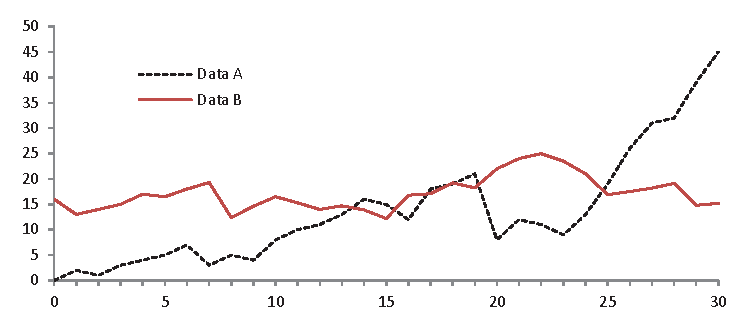
\includegraphics[width=\textwidth]{fig1.eps}
\caption{A figure caption is always placed below the illustration.
Please note that short captions are centered, while long ones are
justified by the macro package automatically.} \label{fig1}
\end{figure}

\begin{theorem}
This is a sample theorem. The run-in heading is set in bold, while
the following text appears in italics. Definitions, lemmas,
propositions, and corollaries are styled the same way.
\end{theorem}
%
% the environments 'definition', 'lemma', 'proposition', 'corollary',
% 'remark', and 'example' are defined in the LLNCS documentclass as well.
%
\begin{proof}
Proofs, examples, and remarks have the initial word in italics,
while the following text appears in normal font.
\end{proof}
For citations of references, we prefer the use of square brackets
and consecutive numbers. Citations using labels or the author/year
convention are also acceptable. The following bibliography provides
a sample reference list with entries for journal
% articles~\cite{ref_article1}, an LNCS chapter~\cite{ref_lncs1}, a
% book~\cite{ref_book1}, proceedings without editors~\cite{ref_proc1},
% and a homepage~\cite{ref_url1}. Multiple citations are grouped
% \cite{ref_article1,ref_lncs1,ref_book1},
% \cite{ref_article1,ref_book1,ref_proc1,ref_url1}.
%
% ---- Bibliography ----
%
% BibTeX users should specify bibliography style 'splncs04'.
% References will then be sorted and formatted in the correct style.
%
\bibliographystyle{splncs04}
\bibliography{mybibliography}
%
\end{document}
